\documentclass[11pt]{scrartcl}
\usepackage[utf8]{inputenc}
\usepackage{amsmath, amssymb, amsthm, bbm}
\usepackage{booktabs, verbatim, graphicx, framed}
\usepackage[sexy, hints]{evan}
\title{Physics with Greenwood}
\author{Anay Aggarwal}

\begin{document}

\maketitle

\section{Homework 1}
Equations
$$v=v_0+at$$
$$x=x_0+v_0t+\frac12 at^2$$
$$v^2=v_0^2+2a\Delta x$$
Homework problems
\begin{example}
  [Problem 2]
\end{example}
\begin{soln}
  We can use
  $$v=\frac{\Delta x}{\Delta t}\implies \Delta t = \frac{\Delta x}{v}$$
  Thus
  $$\Delta t=\frac{15 km}{25 km/h}=\frac{3}{5}h$$
\end{soln}
\begin{example}
  [Problem 5]
\end{example}
\begin{soln}
  We can use
  $$v=\frac{x_2-x_1}{t_2-t_1}=\frac{-4.2cm-3.4cm}{6.1s-3.0s}=\frac{-7.6}{3.1}cm/s$$
\end{soln}
\begin{example}
  [Problem 7]
\end{example}
\begin{soln}
  Notice that, for the first part of the drive,
  $$\Delta t=\frac{\Delta x}{v}=\frac{130km}{95 km/h}=\frac{26}{19}h$$
  The total drive is $3$ hours and $20$ minutes, or $\frac{10}{3}$ hours.
  Hence the time for the second part of the drive is
  $$\frac{10}{3}-\frac{26}{19}=\frac{112}{57}$$
  hours. To find the distance, we can use
  $$v=\frac{\Delta x}{\Delta t}\implies \Delta x=v\Delta t=65 km/h\cdot \frac{112}{57}h=\frac{7280}{57}km$$
  Hence the total distance is
  $$130km+\frac{7280}{57}km\approx 257.72km$$
  Which is the answer to part a of problem $7$.
  For part b, just note that
  $$v=\frac{\Delta x}{\Delta t}\approx \frac{257.72km}{3.3h}\approx 78 km/h$$
\end{soln}
\begin{example}
  [Problem 9]
\end{example}
\begin{soln}
  The total distance is $8\cdot \frac{1}{4}=2$ miles. Hence
  $$|v|=\frac{\Delta x}{\Delta t}=\frac{2 mi}{12.5 min}=0.16 mi/min=4.29 m/s$$
  Which is the average speed. The net displacement is zero, so the average velocity
  in the end is also zero (note that this is not equal to the average speed since velocity
  also contains direction).
\end{soln}
\begin{example}
  [Problem 11]
\end{example}
\begin{soln}
  This one is a bit of a thinking problem. From the reference frame
  of the blue locomotive, the red locomotive is approaching with speed
  $$95km/h-(-95km/h)=190km/h$$
  Hence
  $$v=\frac{\Delta x}{\Delta t}\implies \Delta t=\frac{\Delta x}{v}=\frac{8.5 km}{190 km/h}\approx 0.045 h$$
\end{soln}
\begin{example}
  [Problem 14]
\end{example}
\begin{soln}
  First of all, the net displacement is zero so it follows that the
  average velocity is zero as well. For the average speed, we first need to compute
  the total time taken. For the first section,
  $$\Delta t=\frac{\Delta x}{v}=\frac{250 km}{95 km/h}\approx 2.63 h$$
  For the second part, $\Delta t=1h$. For the third part,
  $$\Delta t=\frac{\Delta x}{v}=\frac{250 km}{55 km/h}\approx 4.55h$$
  Hence $\Delta t_{total}=8.18h$. So
  $$|v|=\frac{500km}{8.18h}\approx 61.12 km/h$$
\end{soln}
\begin{example}
  [Problem 17a]
\end{example}
\begin{soln}
  We can use the kinematics formula
  $$v=v_0+at\implies a=\frac{v-v_0}{t}=\frac{10 m/s}{1.35s}\approx 7.4 m/s^2$$
\end{soln}
\begin{example}
  [Problem 18]
\end{example}
\begin{soln}
  Using the kinematics formula
  $$v=v_0+at\implies t=\frac{v-v_0}{a}=\frac{30 km/h}{1.6 m/s^2}=5.21s$$
\end{soln}
\section{Homework 2}
\begin{example}
  [Problem 22]
\end{example}
\begin{soln}
  We desire acceleration, and we know the distances and velocities, so we can use the equation
  $$v_f^2=v_i^2+2a\Delta x$$
  Isolating $a$,
  $$a=\frac{v_f^2-v_i^2}{2\Delta x}$$
  This is it, since $v_f=0m/s, v_i=23m/s, \Delta x=85m$. Hence
  $$a=\frac{0m^2/s^2-529m^2/s^2}{170m}\approx -3.1 m/s^2$$
  Now for some functional analysis. The units are clearly correct, and the
  sign makes sense since the car is \textit{slowing down}. The magnitude seems reasonable as well.
\end{soln}
\begin{example}
  [Problem 23]
\end{example}
\begin{soln}
  The knowns are acceleration and velocity, and the unknowns are distance and
  time, but we only desire distance. Looking at our kinematics equations,
  the fitting one is
  $$v_f^2=v_i^2+2a\Delta x$$
  $$\Delta x=\frac{v_f^2-v_i^2}{2a}$$
  Reading the problem, $v_f=33m/s, v_i=0m/s, a=3 m/s^2$. Hence
  $$\Delta x=\frac{1089 m^2/s^2-0m^2/s^2}{6 m/s^2}=181.5 m$$
  Units make sense, and the sign makes sense. The result seems practical
  qualitatively.
\end{soln}
\begin{example}
  [Problem 25]
\end{example}
\begin{soln}
  We know all but distance and acceleration. We desire distance.
  First we can use
  $$v_f=v_i+at$$
  $$a=\frac{v_f-v_i}{t}$$
  Then use
  $$v_f^2=v_i^2+2a\Delta x$$
  $$\Delta x=\frac{v_f^2-v_i^2}{2a}=\frac{v_f^2-v_i^2}{2(v_f-v_i)}t=\frac{t}{2}(v_f+v_i)$$
  And $v_i=21m/s, v_f=0m/s, t=6s$. So
  $$\Delta x=21m/s\cdot \frac{6s}{2}=63m$$
  Units check out, sign checks out, qualitatively it makes sense.
\end{soln}
\begin{example}
  [Problem 27]
\end{example}
\begin{soln}
  Since we know the velocities and the distance, we can use
  $$v_f^2=v_i^2+2a\Delta x$$
  $$a=\frac{v_f^2-v_i^2}{2\Delta x}$$
  Since $v_f=0km/h,  v_i=85km/h, \Delta x=0.8m$,
  $$a=-\frac{7225 km^2/h^2}{1.6m}=-348m/s^2=-35g$$
  The sign is correct, the units are correct, and the magnitude makes sense.
\end{soln}
\section{Homework 3}
\textbf{Disclaimer}: In all problems, the positive direction is upwards
and the negative direction is downwards.
\begin{example}
  [Problem 33]
\end{example}
\begin{soln}
  We can use
  $$y_f=y_i+v_it+\frac{1}{2}at^2$$
  $$\Delta y=\frac{1}{2}at^2$$
  Since $v_i=0 m/s$. Since $a=-g=-10 m/s^2$,
  $$\Delta y=-5t^2 m/s^2$$
  And since $t=3.25s$,
  $$\Delta y\approx -52.8m$$
  So the cliff is $52.8m$ high. Functional analysis works.
\end{soln}
\begin{example}
  [Problem 35]
\end{example}
\begin{soln}
  We can use the kinematics equation
  $$\Delta y=v_it+\frac{1}{2}at^2$$
  Since $v_i=0m/s$,
  $$\Delta y=\frac{1}{2}at^2\implies t=\sqrt{\frac{2\Delta y}{a}}$$
  Plugging in $\Delta y=-380m, a=-10m/s^2$, $t\approx 8.7s$.
  For part b, we can use
  $$v_f=v_i+at=0m/s-10m/s^2\cdot 8.7s=-87m/s$$
  Functional analysis works.
\end{soln}
\begin{example}
  [Problem 36]
\end{example}
\begin{soln}
  When it hits its maximum height, the velocity is zero. So
  $$v_i+at=0\implies t=-\frac{v_i}{a}=2.2s$$
  Then
  $$y_f=y_i+v_it+\frac{1}{2}at^2$$
  Plugging,
  $$y_f=24.2m$$
  For part $b$,
  $$\Delta y=v_it-\frac{1}{2}at^2$$
  But $\Delta y=0$, so
  $$v_it=\frac{1}{2}at^2\implies t=\frac{2v_i}{a}=4.4s$$
\end{soln}
\begin{example}
  [Problem 38]
\end{example}
\begin{soln}
  Graphs
  \begin{center}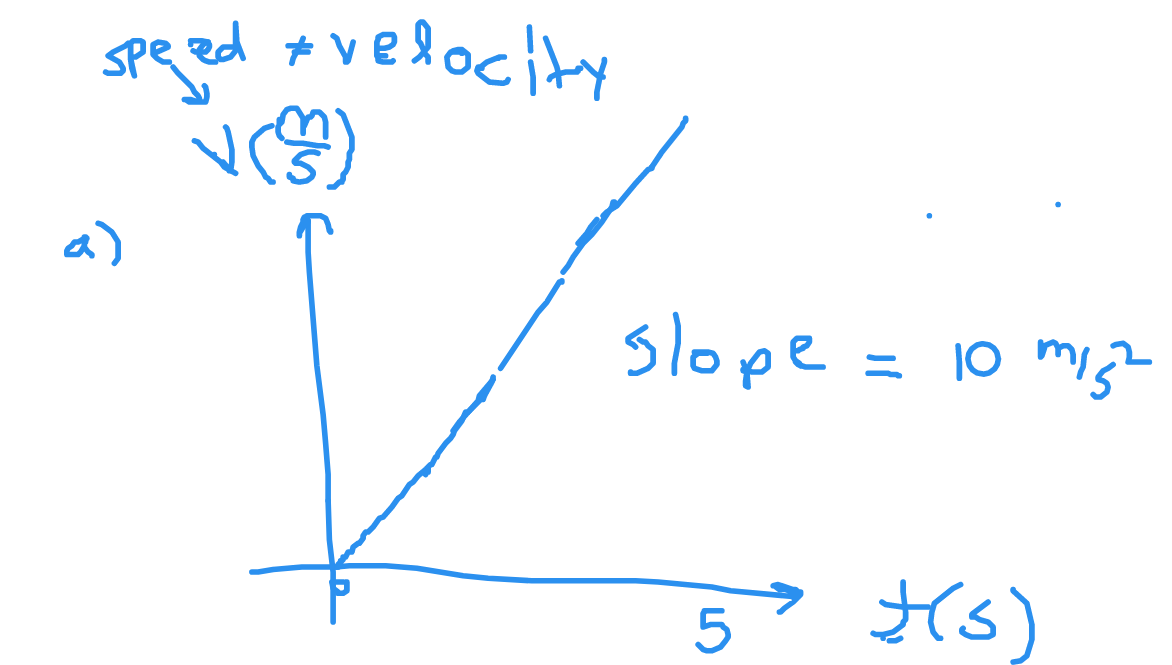
\includegraphics[scale=0.3]{velocity.png}\end{center}
  \begin{center}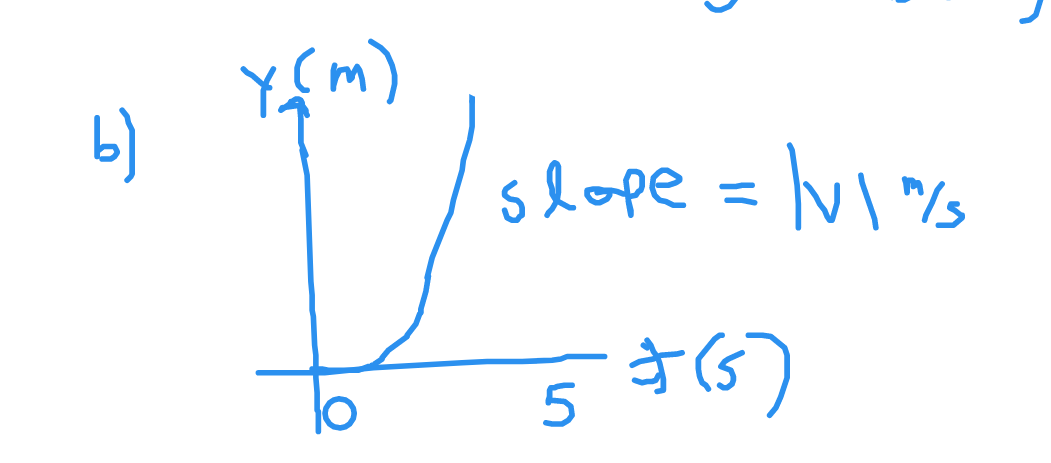
\includegraphics[scale=0.3]{position.png}\end{center}
\end{soln}
\begin{example}
  [Problem 40]
\end{example}
\begin{soln}
  The distance travelled is
  $$\frac{1}{2}at^2$$
  And the result is obvious using
  $$\sum_{k=1}^n 2k-1=n^2$$
\end{soln}
We completed 47 during class time.
\section{Homework 4}
\begin{example}
  Context rich problem (long distance archer)
\end{example}
\begin{soln}
  Denote the positive $y$ direction as downward, and the positive $x$ direction as right.
  The known quantities are $v_{initial}=25m/s$, $v_{initial, y}=0m/s$. Thus $v_{initial, x}=v_{initial}$ is also known.
  We can treat $\theta$ as a known quantity. We want $y_{final}$. The
  relevant equations are the projectile motion equations:
  $$x_f=x_i+v_{ix}t\implies \Delta x=v_{ix} t$$
  $$y_f=y_i\underbrace{+}_{downward}\frac{1}{2}gt^2\implies \Delta y=\frac{1}{2}gt^2$$
  The problem is a bit tricky because it lands on a mountain,
  rather than a flat ground. We know what this is physically,
  but in order to \textit{solve} the problem, we have to represent
  it mathematically. Suppose the peak of the mountain is $A$.
  Suppose the arrow lands on the mountain at point $B$. Draw the triangle as shown:
  \begin{center}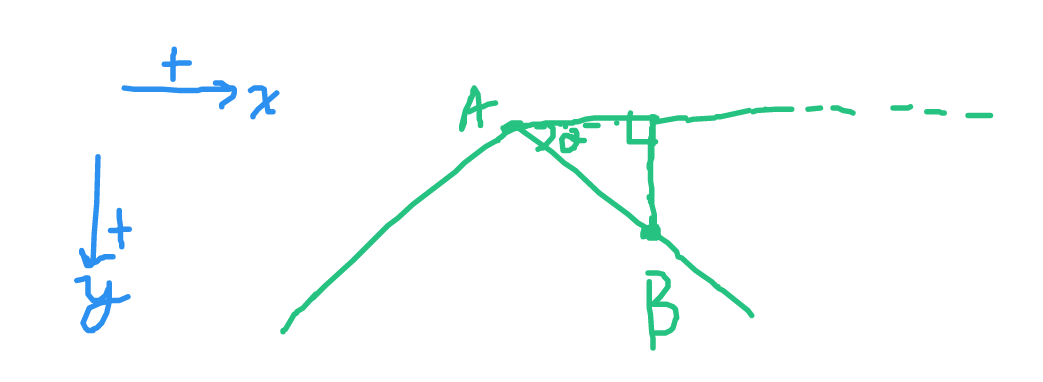
\includegraphics[scale=0.3]{projectile.png}\end{center}
  This diagram shows us that
  $$\tan\theta=\frac{\Delta y}{\Delta x}$$
  In this equation, we can substitute our symbolic expressions for $\Delta x,\Delta y$.
  Therefore,
  $$\tan\theta=\frac{\Delta y}{\Delta x}=\frac{\frac{1}{2}gt^2}{v_{ix}t}=\frac{gt}{2v_i}$$
  $$t=\frac{2v_i\tan\theta}{g}$$
  Now to get $y_{final}$, we can use the second equation. Without loss of generality, suppose $y_i=0 m$. Then
  $$y_f=\frac{1}{2}gt^2=\frac{g}{2}\frac{4v_i^2\tan^2\theta}{g^2}=\frac{2v_i^2\tan^2\theta}{g}$$
  The units here are correct since the numerator has units $m^2/s^2$ and the denominator has units $m/s^2$  so the total units are $m$,
  which is sensible for distance. We can plug in $g\approx 10m/s^2, v_i=25m/s$ to get
  $$y_f=125\tan^2\theta m$$
  Therefore, the projectile falls $125\tan^2\theta$ meters before it hits the mountain. This is in terms of $\theta$
  so we can't do immediate functional analysis. However, we can check limiting cases of $\theta$. If $\theta=0$,
  we get that the projectile falls $0$m, which makes a lot of sense since it starts at the ground and ends at the ground.
  If $\theta=90$, then we get that it falls for infinitely long, which makes sense since you're throwing it from the top of a
  never-ending wall.
\end{soln}
\begin{example}
  Explanation Task (train raindrop)
\end{example}
\begin{soln}
  The basic formula that should be known is
  $$\overrightarrow{v_{RE}}+\overrightarrow{v_{ET}}=\overrightarrow{v_{RT}}$$
  Where $R$ is the raindrop, $E$ is the earth, and $T$ is the train. We also know that the two legs of a $45-45-90$ triangle are equal.
  Drawing the vectors out, we get the following diagram:
  \begin{center}\includegraphics[scale=0.3]{relative.png}\end{center}
  This tells us that $|\overrightarrow{v_{RE}}|=|\overrightarrow{v_{ET}}|$ from 45-45-90 triangles. In the question, $|\overrightarrow{v_{ET}}|=|\overrightarrow{v_{TE}}|=|\overrightarrow{v_T}|$.
  Hence the velocity of the rain is equal to the velocity of the earth. This makes sense using the fundamental theorem of thinking.
\end{soln}
\end{document}
